% Author: Izaak Neutelings (September 2020)
\documentclass[border=3pt,tikz]{standalone}
\usepackage{amsmath}
\usepackage{tikz}
\usepackage{physics}
\usetikzlibrary{calc}
\usetikzlibrary{bending} % for arrow head angle
\usetikzlibrary{patterns}
\usetikzlibrary{decorations.pathmorphing} % for decorate random steps
\tikzset{>=latex} % for LaTeX arrow head
\usepackage{xcolor}

\colorlet{xcol}{blue!70!black}
\colorlet{vcol}{green!45!black}
\tikzstyle{vvec}=[->,very thick,vcol,line cap=round]
\tikzstyle{ground}=[preaction={fill,top color=black!10,bottom color=black!5,shading angle=20},
                    fill,pattern=north east lines,draw=none,minimum width=0.3,minimum height=0.6]
\tikzstyle{mass}=[line width=0.5,red!30!black,fill=red!40!black!10,rounded corners=1,
                  top color=red!40!black!20,bottom color=red!40!black!10,shading angle=20]
\def\car{
  \draw[thick,rounded corners=2,orange!60!black,
        top color=orange!70!black!6,bottom color=orange!70!black!2,shading angle=10]
    (0,1.1*\CR) rectangle++ (\CW,\CH);
  \fill[black!20]
    (0.15*\CW,\CR) circle(\CR) (0.85*\CW,\CR) circle(\CR);
  \draw[black,fill=black!90,thin,even odd rule]
    (0.15*\CW,\CR) circle(\CR) circle(0.5*\CR)
    (0.85*\CW,\CR) circle(\CR) circle(0.5*\CR);
}

\begin{document}


% STATIONARY REFERENCE FRAME
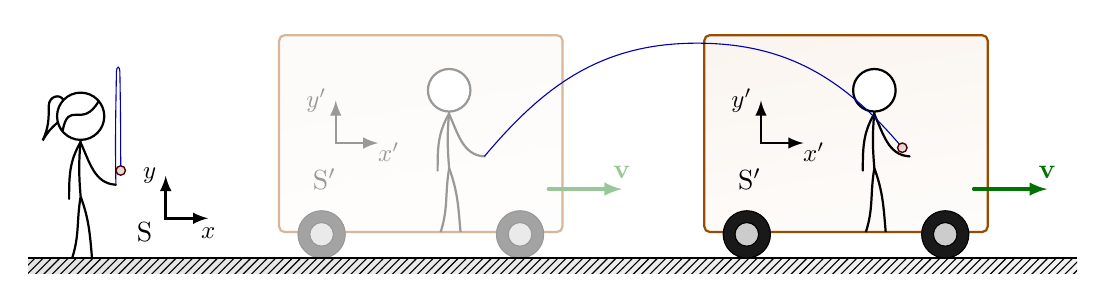
\begin{tikzpicture}
  \def\r{0.06}    % mass radius
  \def\H{1.8}     % human height
  \def\CW{3.6}    % car width
  \def\CH{2.5}    % car height
  \def\CR{0.3}    % wheel radius
  \def\d{0.5*\CW} % car distance
  \def\W{3.7*\CW} % ground width
  \def\D{0.2}     % ground depth
  
  % SETUP
  \draw[ground] (-0.05*\W,0) rectangle++ (\W,-\D);
  \draw (-0.05*\W,0) --++ (\W,0);
  
  % PERSON 1
  \coordinate (H) at (0,\H);
  \draw[thick,line cap=round]
    (H)++(-165:0.3) to[out=-140,in=60]++ (-130:0.3)
    to[out=65,in=-90,looseness=1.0]++ (80:0.45) to[out=90,in=120,looseness=1.4]++ (20:0.2); % pony tail
  \draw[thick,fill=white] (H) circle (0.3);
  \draw[thick,line cap=round] (H)++(-140:0.3) to[out=80,in=-120,looseness=1.8]++ (40:0.6); % hair
  \draw[thick] (H)++(-90:0.3) coordinate (N) to[out=-95,in=95]++ (0,-0.40*\H) coordinate (P);
  \draw[thick,line cap=round] (N)++(-95:0.03) to[out=-65,in=177]++ (0.25*\H,-0.3*\H) coordinate (RH);
  \draw[thick,line cap=round] (N)++(-95:0.03) to[out=-120,in=90]++ (-0.08*\H,-0.4*\H);
  \draw[thick] (P) to[out=-70,in=95] (0.08*\H,0);
  \draw[thick] (P) to[out=-100,in=72] (-0.06*\H,0);
  
  % PROJECTILE 1
  \draw[very thin,xcol,line width=0.4] %,dashed
    (RH) to[out=91,in=-91]++ (0.004*\H,0.8*\H) arc(179:2:{0.012*\H} and 0.03*\H)
         to[out=-89,in=90]++ (0.006*\H,-0.7*\H) coordinate (M);
  \draw[mass] (M) circle(\r); %node[right] {$m$};
  
  % AXIS 1
  \node (A) at (0.45*\H,0.18*\H) {S};
  \draw[<->,line width=0.9]
    (A)++(0.15*\H,0.4*\H) node[left,scale=0.9] {$y$} |-++
         (0.3*\H,-0.3*\H) node[below,scale=0.9] {$x$};
  
  % CAR 1
  \begin{scope}[shift={(0.7*\CW,0)}]
    \car
    \draw[thick,fill=white] (0.6*\CW,\H+\CR+0.03) circle (0.15*\H) coordinate (H);
    \draw[thick] (H)++(-90:0.15*\H) coordinate (N) to[out=-95,in=95]++ (0,-0.40*\H) coordinate (P);
    \draw[thick,line cap=round] (N)++(-95:0.03) to[out=-65,in=177]++ (0.25*\H,-0.3*\H) coordinate (RH1);
    \draw[thick,line cap=round] (N)++(-95:0.03) to[out=-120,in=90]++ (-0.08*\H,-0.4*\H);
    \draw[thick] (P) to[out=-70,in=95] ($(H)+(0.08*\H,-\H)$);
    \draw[thick] (P) to[out=-100,in=72] ($(H)+(-0.06*\H,-\H)$);
    \node at (0.16*\CW,0.4*\CH) {S$'$};
    \draw[<->,line width=0.9]
      (0.2*\CW,0.8*\CH) node[left,scale=0.9] {$y'$} |-++
      (0.3*\H,-0.3*\H) node[below right=-3.5,scale=0.9] {$x'$};
    \draw[vvec] (0.95*\CW,0.35*\CH) --++ (0.26*\CW,0) node[above] {$\vb{v}$};
    \fill[white,opacity=0.6] (-0.05*\CW,0) rectangle++ (1.3*\CW,1.05*\CH+\CR);
    \draw (-0.1*\CW,0) --++ (1.45*\CW,0);
  \end{scope}
  
  % CAR 2
  \begin{scope}[shift={(1.7*\CW+\d,0)}]
    \car
    \draw[thick,fill=white] (0.6*\CW,\H+\CR+0.03) circle (0.15*\H) coordinate (H);
    \draw[thick] (H)++(-90:0.15*\H) coordinate (N) to[out=-95,in=95]++ (0,-0.40*\H) coordinate (P);
    \draw[thick,line cap=round] (N)++(-95:0.03) to[out=-65,in=177]++ (0.25*\H,-0.3*\H) coordinate (RH2);
    \draw[thick,line cap=round] (N)++(-95:0.03) to[out=-120,in=90]++ (-0.08*\H,-0.4*\H);
    \draw[thick] (P) to[out=-70,in=95] ($(H)+(0.08*\H,-\H)$);
    \draw[thick] (P) to[out=-100,in=72] ($(H)+(-0.06*\H,-\H)$);
    \node at (0.16*\CW,0.4*\CH) {S$'$};
    \draw[<->,line width=0.9]
      (0.2*\CW,0.8*\CH) node[left,scale=0.9] {$y'$} |-++
      (0.3*\H,-0.3*\H) node[below right=-3.5,scale=0.9] {$x'$};
    \draw[vvec] (0.95*\CW,0.35*\CH) --++ (0.26*\CW,0) node[above] {$\vb{v}$};
  \end{scope}
  
  % PROJECTILE 2
  \draw[very thin,xcol,line width=0.4] %,dashed
    (RH1) to[out=50,in=180]++ (0.5*\CW+0.5*\d,\CH-0.59*\H)
          to[out=0,in=130] ($(RH2)+(130:0.08*\H)$) coordinate (M);
  \draw[mass] (M) circle(\r); %node[right] {$m$};
  
\end{tikzpicture}


\end{document}